\documentclass[22pt]{beamer}
\usepackage[orientation=portrait, size=custom, width=91.44, height=91.44,scale=1.2]{beamerposter} % 36in*2.5 = 90cm
\usepackage[absolute,overlay]{textpos}
\usepackage{bookmark} %pdflatex says to use this to avoid errors...
\usepackage{graphicx} %for including images
\graphicspath{{figs/}} %location of images
\usepackage{wrapfig} %wrap text around the images
\usepackage{listingsutf8}    %package for code environment; use this instead of verbatim to get automatic line break; use this instead of listings to get (•)
\usepackage{amsmath}
\usepackage{gensymb}
\usepackage[export]{adjustbox}
\usepackage[skins,theorems]{tcolorbox}
\usepackage{tikz}
\newcommand*\circled[1]{\tikz[baseline=(char.base)]{
            \node[shape=circle,draw,inner sep=2pt] (char) {#1};}}
\usepackage{array}
\usepackage{booktabs,adjustbox}
\usepackage{subcaption} 



%\mode<presentation>
%this doesn't seem to make any difference; leave for now for trying out
\usetheme{Berlin}
\definecolor{MacBlue}{rgb}{0.10196,0.22353,0.53725}
\definecolor{MacMaroon} {rgb}{0.47843, 0, 0.23137}
\definecolor{MacMaroon2} {rgb}{0.47451, 0, 0}
\definecolor{MacGray}{rgb}{0.50196,0.49804,0.51765}
\definecolor{MacMaroon3}{rgb}{00.47,0.2,0.31}
\definecolor{MacGold}{rgb}{1, 0.75,0.35}
\usecolortheme[named=MacMaroon2]{structure}
\setbeamertemplate{caption}[numbered]
\setbeamertemplate{navigation symbols}{}

\title{Pillbox: Bringing Patient Experiences into the 21st Century}
%\subtitle{}  
  \author[Santana, Santana, Khan \& Khedri]{Carlos Santana, Cesar Santana, Madeeha Khan, Ridha Khedri$^\dagger$ \vspace{0.3cm} \newline \small \{khanm57, santanca, santanjc\}@mcmaster.ca}
  \institute[McMaster University]{$^\dagger$Department of Computing and Software, McMaster University}
  \date{December 5, 2018}

\begin{document}
%compile with pdflatex

%there is only one frame, because there is only one page; yeah, it's a poster
%textblock and block seem to work nicely to organize layout
\begin{frame}[fragile]

\begin{textblock}{2}(0.7,1)

\includegraphics[height=8.5cm]{englogo.png} % We can use CAS logo as well? 
\end{textblock}

\begin{textblock}{2}(12.1,1)

\includegraphics[height=7cm, width=20cm]{pillbox_logo.png}
\end{textblock}

\begin{textblock}{8}(4,1)
\titlepage
\end{textblock}

\begin{textblock}{7.25}(0.5,3.1)

%this needs help
\begin{block}{Introduction}
The idea behind Pillbox is to build an application which will help patients and pharmacists better keep track of medication dispensary and usage. The application is mainly geared towards patients, and will serve a wide range of users, including the elderly and children. \\
Nowadays, pharmacies have high-tech methods of dispensing, counting, and keeping track of medications and prescriptions. However, the user experience for patients has remained stagnant. Patients still need to count their own remaining medication, set various alarms, and communicating with healthcare professionals is more cumbersome than it should be.\\
Pillbox will use the latest technology available to make the patient experience as secure, efficient, and user-friendly as possible.
\end{block}

\begin{block}{Target User Base}
The target audience of the application are people who use medication regularly. It is directed especially to those who experience chronic illnesses, the elderly and/or anyone who may need assistance taking medication. The goal for the application is to be easily accessible and effortless to use, as well as low in data, storage. 
\end{block}

\begin{block}{Use Case UML Diagram}

\begin{figure}
\begin{center}
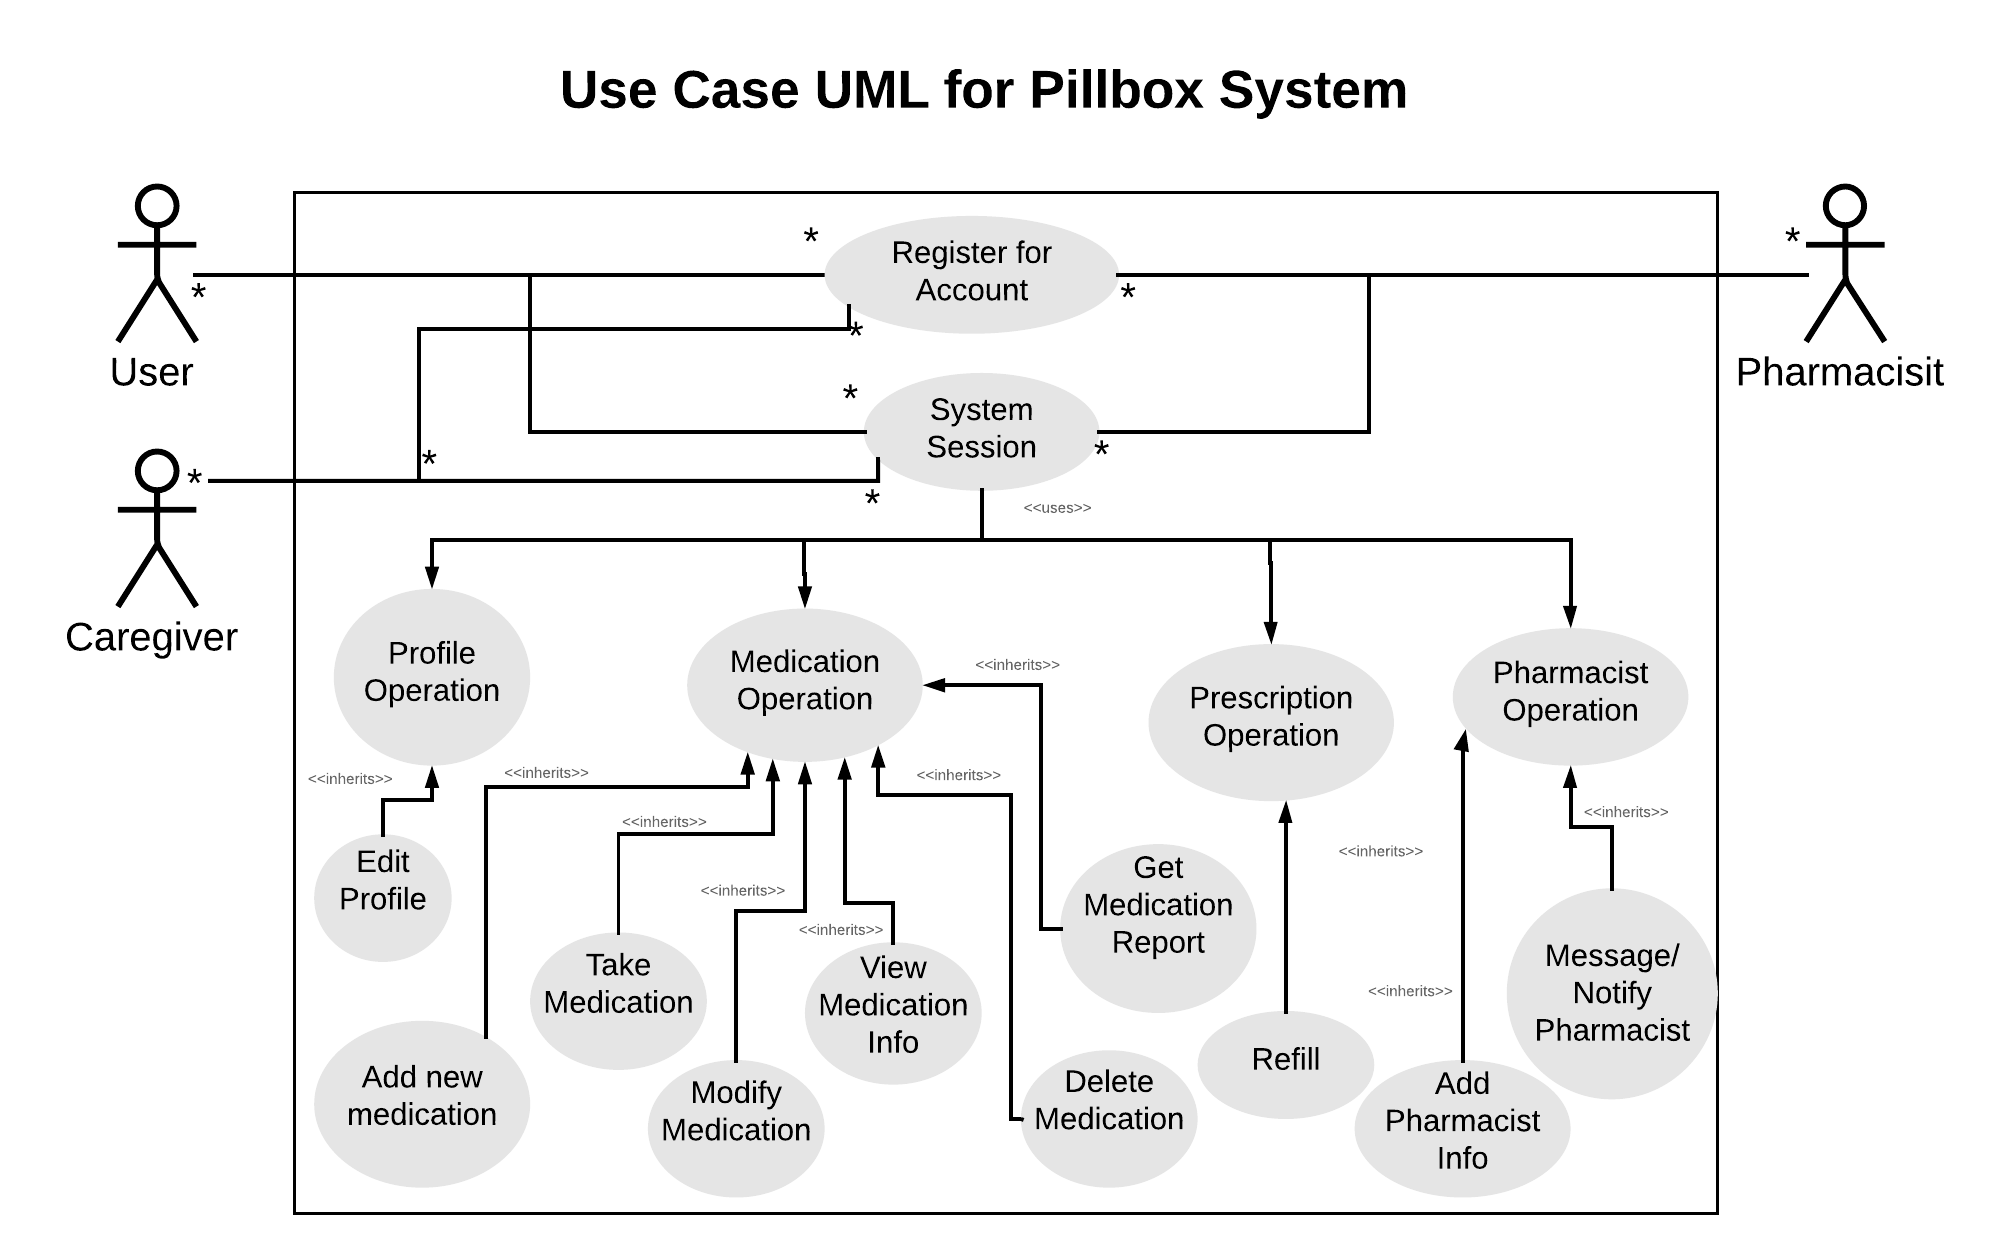
\includegraphics[height=25cm, width=40cm]{UseCaseUML.png}
\end{center}
\caption{Use Case Diagram for the Pillbox system. }
\end{figure}
The above diagram illustrates the three actors and their role with interacting with the system. An actor is a role played by one of three users:
\begin{itemize} 
\item the user, who can view their medication information, adding new prescriptions, receive reminders to take medication and add pharmacy information. 
\item the caregiver, whose role is to reduce the isolation that patients may feel
\item the pharmacist,  so the user can build a trusting relationship with their pharmacist, and can easily ask any questions and bring up any concerns they may have. 
\begin{itemize}
\item This, we think, is essential, as patients who have a follow-up with their healthcare professional discontinue medication a little less that 50\%  \cite{selmesmitchell2007} less often that patients who do not.
\end{itemize}

%\cite{selmesmitchell2007} ***********************************************

\end{itemize}

Pillbox aims to make the experience of taking regular medications, which patients can find isolating, confusing, and stigmatizing, and incorporate more guidance and support.  \\

\end{block}
\end{textblock}



\begin{textblock}{7.25}(8.25,3.1)
\begin{block}{Competitive Analysis for Pillbox}
The Medisafe and MyTherapy apps have over 1 million downloads each on the Play Store. While these apps may be simple and easy to use they lack some key features that would be needed by many who use medication on a daily basis. The chart below illustrates some of these key features.



\begin{center}
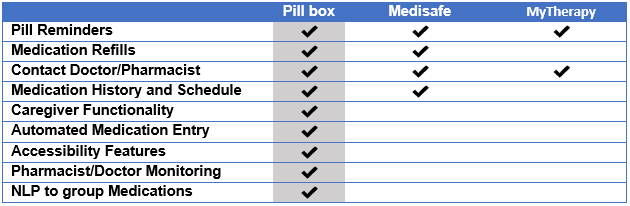
\includegraphics[height=10.5cm]{CompetitiveAdvantage.png}
\end{center}
Patients who fill their prescriptions often have a difficult time understanding prescription instructions, keeping track of their intake, and integrating their medication into their lives with the least amount of intrusion.\\
Pillbox has integrated features to solve many of the problems that result in discontinuity of medication by the patient.
\end{block}

\begin{block}{User Survey Results}

\begin{figure}
\begin{center}
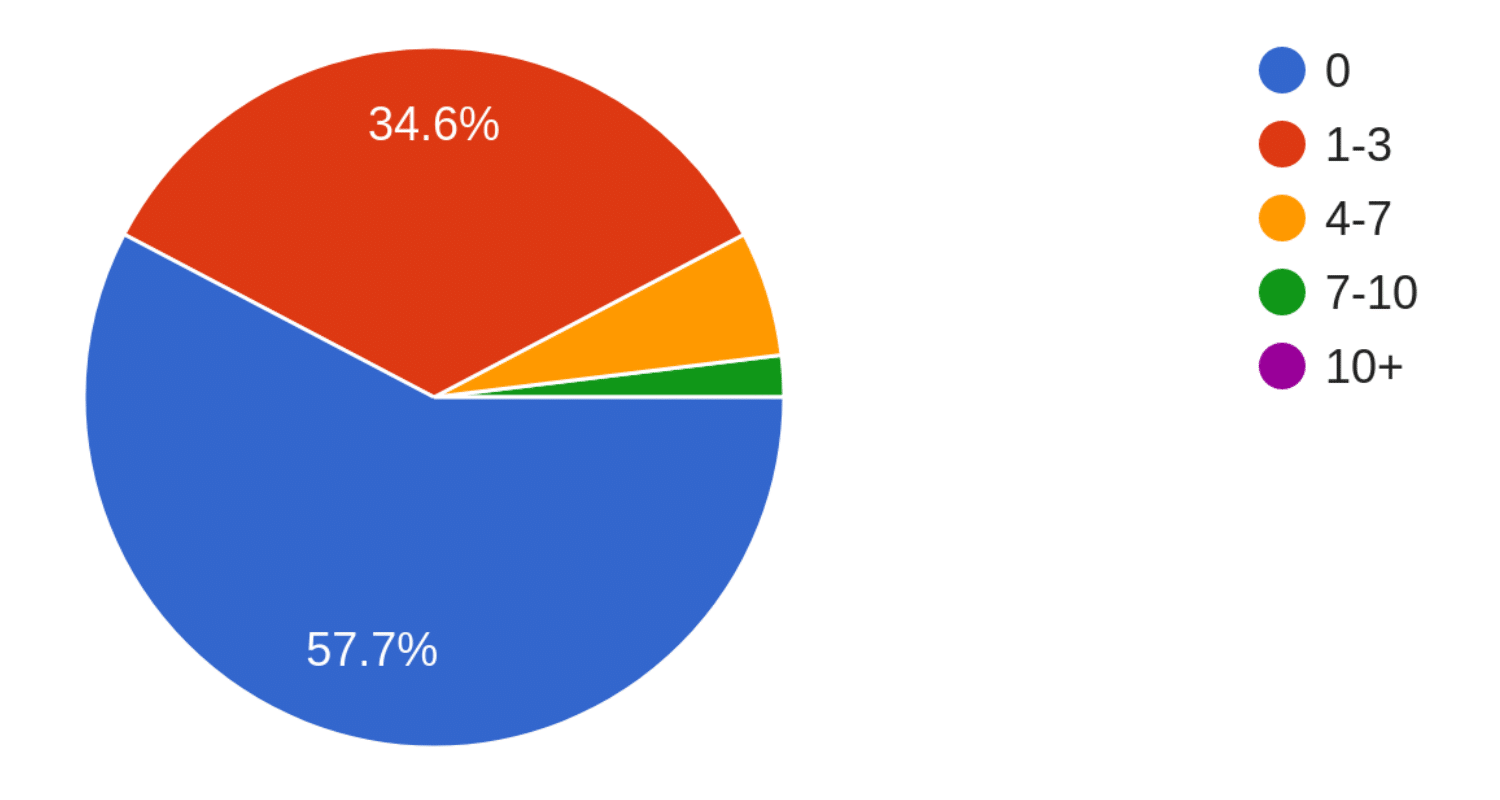
\includegraphics[height=12cm, width=25cm]{medications.png}
\end{center}
\caption{Pie chart with results from the survey question "How many medications (prescription or otherwise) have you taken regularly for the past three months?". }
\end{figure}
This graph illustrates how many medications the participants take regularly. Evidently, more than half the sampling takes none, but this is a function of the audience the survey reached -- mostly younger people, who do not have health issues. 
\\However, for the users who take even more than 2 or 3 medications, Pillbox could be extremely useful, since these may be medications with hard to remember instructions, or may require the user to ask their pharmacist for a lot of clarification.
\end{block}

\begin{block}{Conclusions \& Future Work}
The design allows for medication users, the pharmacist, and caregivers to be involved in the medication process. Pillbox is ready to start designing and implementing the solution. We intend on creating the mobile application and having it ready for testing by early 2019. There is always room to improve and we always want to integrate features that would be beneficial for users.
\end{block}


\begin{block}{Acknowledgements}
The Pillbox team would like to thank Dr. Kehdri for all his help and guidance.
\end{block}


\begin{block}{References}
\setbeamertemplate{bibliography item}{\insertbiblabel}
\bibliographystyle{ieeetr}
{\scriptsize
\bibliography{bib}}
\end{block}


\end{textblock}


\end{frame}
\end{document}
